\documentclass[letterpaper,11pt]{article}

\usepackage{latexsym}
\usepackage[empty]{fullpage}
\usepackage{titlesec}
\usepackage{marvosym}
\usepackage[usenames,dvipsnames]{color}
\usepackage{verbatim}
\usepackage{enumitem}
\usepackage[hidelinks]{hyperref}
\usepackage{fancyhdr}
\usepackage[english]{babel}
\usepackage{tabularx}
\usepackage{fontawesome5}
\usepackage{multicol}
\setlength{\multicolsep}{-3.0pt}
\setlength{\columnsep}{-1pt}
\input{glyphtounicode}

%new packages

\usepackage{fontenc}
\usepackage{amsmath}
\usepackage{amssymb}
\usepackage{graphicx}



%----------FONT OPTIONS----------

\pagestyle{fancy}
\fancyhf{} % clear all header and footer fields
\fancyfoot{}
\renewcommand{\headrulewidth}{0pt}
\renewcommand{\footrulewidth}{0pt}

% Adjust margins
\addtolength{\oddsidemargin}{-0.6in}
\addtolength{\evensidemargin}{-0.5in}
\addtolength{\textwidth}{1.19in}
\addtolength{\topmargin}{-.7in}
\addtolength{\textheight}{1.4in}

\urlstyle{same}

\raggedbottom
\raggedright
\setlength{\tabcolsep}{0in}

% Sections formatting
\titleformat{\section}{
  \vspace{-4pt}\scshape\raggedright\large\bfseries
}{}{0em}{}[\color{black}\titlerule \vspace{-5pt}]



% Ensure that generate pdf is machine readable/ATS parsable
\pdfgentounicode=1

%-------------------------
% Custom commands
\newcommand{\resumeItem}[1]{
  \item\small{
    {#1 \vspace{-2pt}}
  }
}

\newcommand{\classesList}[4]{
    \item\small{
        {#1 #2 #3 #4 \vspace{-2pt}}
  }
}

\newcommand{\resumeSubheading}[4]{
  \vspace{-2pt}\item
    \begin{tabular*}{1.0\textwidth}[t]{l@{\extracolsep{\fill}}r}
      \textbf{#1} & \textbf{\small #2} \\
      \textit{\small#3} & \textit{\small #4} \\
    \end{tabular*}\vspace{-7pt}
}

\newcommand{\resumeSubSubheading}[2]{
    \item
    \begin{tabular*}{0.97\textwidth}{l@{\extracolsep{\fill}}r}
      \textit{\small#1} & \textit{\small #2} \\
    \end{tabular*}\vspace{-7pt}
}

\newcommand{\resumeProjectHeading}[2]{
    \item
    \begin{tabular*}{1.001\textwidth}{l@{\extracolsep{\fill}}r}
      \small#1 & \textbf{\small #2}\\
    \end{tabular*}\vspace{-7pt}
}


\newcommand{\resumeSubItem}[1]{\resumeItem{#1}\vspace{-4pt}}

\renewcommand\labelitemi{$\vcenter{\hbox{\tiny$\bullet$}}$}
\renewcommand\labelitemii{$\vcenter{\hbox{\tiny$\bullet$}}$}

\newcommand{\resumeSubHeadingListStart}{\begin{itemize}[leftmargin=0.0in, label={}]}
\newcommand{\resumeSubHeadingListEnd}{\end{itemize}}
\newcommand{\resumeItemListStart}{\begin{itemize}}
\newcommand{\resumeItemListEnd}{\end{itemize}\vspace{-5pt}}

\begin{document}
\fontfamily{cmr}\selectfont
\begin{center}
\parbox{3.0cm}{%
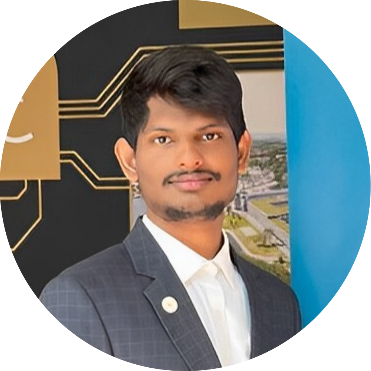
\includegraphics[width=2.7cm,clip]{images/resume_pic_m.png}}
\parbox{\dimexpr\linewidth-3.8cm\relax}{
\vspace{-20pt}
\begin{tabularx}{\linewidth}{L r} \\
    {\Huge \scshape  Venkata Sai Yakkshit Reddy Asodi}~
    \href{https://www.cedzlabs.com/yakkshit}{\vspace{1pt}}\\
      Berlin, Germany. \\ \vspace{1pt}
     \small \raisebox{-0.1\height}\faPhone\ +91 8179936156 ~ \href{mailto:saiyakkshit2001@gmail.com}{\raisebox{-0.2\height}\faEnvelope\  {saiyakkshit2001@gmail.com}} ~ 
    \href{https://linkedin.com/in/yakkshit/}{\raisebox{-0.2\height}\faLinkedin\ {yakkshit}}  ~
    \href{https://yakkshit.com/}{\raisebox{-0.2\height}\faGlobe\ {yakkshit.com}}  ~
    \href{https://github.com/yakkshit}{\raisebox{-0.2\height}\faGithub{ yakkshit}}
    \vspace{-8pt}
\end{tabularx}
}
\end{center}

\vspace{-23pt}
%-----------SUMMARY-----------
\href{https://www.yakkshit.com/#details}{\section{Summary \faLink}
Dynamic Data Engineer with expertise in developing and maintaining data pipelines and microservices. Proven ability in Python development and modern data engineering technologies. Passionate about driving efficiency and enhancing user experiences in data-driven environments.}

%-----------TECHNICAL SKILLS-----------
\section{\href{https://www.linkedin.com/in/yakkshit/details/skills/}{Technical Skills} \faLink}
\begin{itemize}[leftmargin=0.15in, label={}]
\small{\item{
\textbf{Data Engineering - }{AWS, Airflow, dbt, Snowflake, Kafka.} \\
\textbf{Languages - }{Python, SQL, JavaScript.} \\
\textbf{Tools - }{Git, Postman, Swagger.} \\
\textbf{Deployment - }{Docker, Kubernetes.}\\
}}
\end{itemize}
\vspace{-10pt}

%-----------EXPERIENCE-----------
\section{Experience \faLinkedin}
\resumeSubHeadingListStart

\resumeSubheading
{\large Circleup AG \faBuilding}{January 2024 -- July 2024}
{Lead Full Stack Engineer (Data Focus)}{\faMapMarker \hspace{0.1cm} Switzerland}\\
\vspace{10pt}
\textbf{Responsibilities:}
\resumeItemListStart
\resumeItem{Developed and maintained data ingestion pipelines, ensuring data quality and governance. Collaborated with Data Science to implement AI-based solutions, enhancing product features.}
\resumeItem{Designed observability frameworks to monitor data pipelines, optimizing performance and troubleshooting issues.}
\resumeItem{Trained cross-functional teams on data tools and features, promoting data-driven decision-making across the organization.}
\resumeItemListEnd
\vspace{-3pt}
\textbf{Environment:}\emph{AWS, Airflow, Python, Snowflake, Docker, Agile methodologies.}

\resumeSubheading
{Spoki \faBuilding}{Jan 2023 -- May 2024}
{Software Developer}{\faMapMarker \hspace{0.1cm} Italy}\\
\vspace{10pt}
\textbf{Responsibilities:}
\resumeItemListStart
\resumeItem{Developed data-driven web applications using the Meteor framework, integrating complex APIs for data processing and visualization.}
\resumeItem{Led the implementation of data pipelines for analytics, ensuring scalability and performance in high-demand environments.}
\resumeItemListEnd
\vspace{-3pt}
\textbf{Environment:}\emph{Meteor, React, Python, RESTful APIs, Agile methodologies.}

\resumeSubheading
{Cedzlabs \faBuilding}{March 2023 -- July 2024}
{Data Engineer}{\faMapMarker \hspace{0.1cm} India.}\\
\vspace{10pt}
\textbf{Responsibilities:}
\resumeItemListStart
\resumeItem{Designed and implemented data visualization tools, improving user insights and decision-making processes. Collaborated with data teams to ensure integration and functionality of analytics tools.}
\resumeItemListEnd
\vspace{-3pt}
\textbf{Environment:}\emph{React, Python, SQL, Figma, Git.}

\resumeItem{\textbf{\href{https://linkedin.com/in/yakkshit}{Checkout my other experiences by clicking here}}}
\vspace{-5pt}

%-----------PROJECTS-----------
\section{Projects \faGithub}
\vspace{-5pt}
\resumeSubHeadingListStart
\resumeProjectHeading
{\textbf{\href{https://ui.cedzlabs.com/resume}{AI Resume Tuner}} $|$ \emph{Azure Cloud, Next.js, RAG, LLMs}}{August 2023 $|$ \faBuilding \hspace{0.1cm}Microsoft}\\
\vspace{6pt}
\textbf{Description:}
\vspace{-5pt}
\resumeItemListStart
\resumeItem{Developed an AI-powered resume tuner that customizes resumes based on job descriptions. The project utilized Retrieval Augmented Generation and multimodal LLMs, deployed on Azure Cloud for scalability and performance.}
\resumeItemListEnd
\vspace{4pt}
\textbf{Tools:}\emph{
Next.js, Azure Cloud, RAG, LLMs, Microsoft AI Studio.}
\vspace{-10pt}

\resumeProjectHeading
{\href{https://yakkshit.com}{\textbf{Portfolio Website}} $|$ \emph{NextJS, AWS}}{January 2023}\\
\vspace{6pt}
\textbf{Description:}
\vspace{-5pt}
\resumeItemListStart
\resumeItem{Built a portfolio website with secure file encryption on AWS, showcasing projects and skills. Utilized NextJS for performance optimization and React for dynamic UI/UX.}
\resumeItemListEnd
\vspace{4pt}
\textbf{Tools:}\emph{NextJS, AWS, Figma, React.}
\vspace{-12pt}

%-----------ACHIEVEMENTS---------------
\section{Achievements / Extracurricular / Contributions}
\resumeSubHeadingListStart
\resumeItemListStart
\resumeItem{Implemented Agile methodologies in project management, enhancing team collaboration and efficiency.}
\resumeItem{Contributed to open-source projects in data engineering and visualization.}
\resumeItem{Regular participant in tech meetups, focusing on data engineering best practices.}
\resumeItemListEnd

\resumeSubHeadingListEnd
\textbf{Strengths : }\emph{Leadership, problem-solving, attention to detail, and effective communication.} \\

\vspace{10pt}
\end{document}